% !TEX root = ../CINTA-cn.tex
%%%%%%%%%%%%%%%%%%%%%%%%%%%%%%%%%%%%%%%%%%%%%%%%%%%%%%%%%%%%%%%%%%%%
% Author: Libin Wang
% Chapter 11. Quadratic Residues
% This document was released as open source on 2026-06-18.
% Copyright 2023, Libin Wang. Creative Commons License
% This work is licensed under a Creative Commons Attribution-NonCommercial-NoDerivatives 4.0 International License.
%%%%%%%%%%%%%%%%%%%%%%%%%%%%%%%%%%%%%%%%%%%%%%%%%%%%%%%%%%%%%%%%%%%%

\chapter{二次剩余}
\label{chap:qr} 

\begin{introduction}
  \item 二次剩余
  \item 勒让德符号
  \item  欧拉准则
  \item 二次互反律
\end{introduction}

\section{二次剩余与二次非剩余}
\label{sec:qr_qnr}
设$p$是一个奇素数，$a$是与$p$互素的整数，$a$是否是模$p$的平方数？
换而言之，需要判断是否存在$x\in \Z$使得：
\[ x^2 \equiv a \pmod{p}\]
这就是本章的重点主题。

表面上看，这似乎很容易，正如我们之前曾经做过的，只需要把$1$到$p-1$之间的数做平方， 然后看是否有一个数会等于$a$。

\begin{example}
设$p = 11$，$a = 5$，判断$a$是否模$p$的平方数。
只需要写一个简单的 Python 程序，对$1$到$10$之间的数做平方。
\begin{lstlisting}[language=Python]
p = 11
for i in range(1, p):
    print(pow(i, 2, p), end=' ')
print(end='\n')
\end{lstlisting}
得到的输出是：
\[1, 4, 9, 5, 3, 3, 5, 9, 4, 1\]
根据输出可以知道：
\[ 4^2 \equiv 5 \pmod{p}\text{，并且}\quad 7^2 \equiv 5 \pmod{p}\text{。}\] 
 \end{example}
  
当然，穷举法不是我们想要的，知道求解的命令也远远不够，我们想要讨论的比这复杂得多。然而通过这些简单代码和命令我们可以获取数据，从而发现某些模式或者规律，
再从中发现更有价值的解决方案。例如，如果分别设$p = 5, 7, 13$，获得的数据可显示如下：

\begin{minipage}{\textwidth}
	\begin{minipage}[h]{0.3\textwidth}
		\centering
		\begin{tabular}{ | c | c |}
			\hline
			$a$  & $a^2$  \\ \hline
			1 & 1  \\ \hline
			2 & 4  \\ \hline 
			3 & 4 \\ \hline
			4 & 1 \\ \hline 
		\end{tabular}  
			\captionsetup{type=table,hypcap=false}\caption{$a^2 \bmod 5$}
		\label{tab:p_eq_5} 
	\end{minipage}
	\begin{minipage}[h]{0.3\textwidth}
		\centering
	\begin{tabular}{ | c | c |}
		\hline
		$a$  & $a^2$\\ \hline
		1 & 1  \\ \hline
		2 & 4 \\ \hline
		3 & 2  \\ \hline
		4 & 2  \\ \hline
		5 & 4  \\ \hline
		6 & 1  \\ \hline
	\end{tabular}  
	\captionsetup{type=table,hypcap=false}\caption{$a^2 \bmod 7$}
\label{tab:p_eq_7} 
	\end{minipage}
	\begin{minipage}[h]{0.3\textwidth}
		\centering
	\begin{tabular}{ | c | c |}
		\hline
		$a$  & $a^2$ \\ \hline
		1 & 1   \\ \hline
		2 & 4  \\ \hline
		3 & 9  \\ \hline
		4 & 3  \\ \hline
		5 & 12 \\ \hline
		6 & 10 \\ \hline
		7 & 10  \\ \hline
		8 & 12 \\ \hline
		9 &  3 \\ \hline
		10 & 9  \\ \hline
		11 & 4 \\ \hline
		12 & 1 \\ \hline
	\end{tabular}
  \captionsetup{type=table,hypcap=false}\caption{$a^2 \bmod 13$}
  \label{tab:p_eq_13} 
	\end{minipage}
\end{minipage}
 
从上表中我们可以发现什么规律呢？例如，考虑所有表格最后一行，会得到这样一个结论：
 \[(p-1)^2 \equiv 1 \pmod{p} \] 
 为什么呢？很容易证明： 
 \[(p-1)^2 = p^2 - 2p + 1 \equiv 1 \pmod{p}\] 
 这个规律意味着同余式$x^2 \equiv 1 \pmod{p}$有两个解$1$和$p - 1$。
 这是我们已经知道的结论，参看命题~\ref{pro:inv_mod_prime}。况且，$p - 1$不就是模$p$意义下的$-1$？
 
另一个更具一般性的有趣结论是，所有表格的第二列都呈现一种“翻转对称性”，也就是说，如果你把上面表格从中间
对折，平方数部分竟然是重合的。用公式表达如下：
 \[(p - a)^2 \equiv a^2 \pmod{p}\]
 证明与上类似，展开$(p - a)^2$，
 \[(p - a)^2  = p^2 - 2pa + a^2\]
 
 记$b = a^2 \bmod p$，此时同余式$x^2 \equiv b \pmod{p}$有解，
 则必然是两个不同余的解：$a$和$p - a$。$p - a$不就是模$p$意义下的$-a$？
 注意，$p-a \equiv a \pmod{p}$当且仅当$a = 0$。
 把这个结论写成命题如下。

 \begin{proposition}{}{num_qr}
 %\label{prop:num_qr}
 设$p$是一个奇素数，$b$是不被$p$整除的整数。则同余式
 \[x^2 \equiv b \pmod{p} \]
或者没有解，或者有且仅有两个模$p$非同余解。
 \end{proposition}

\begin{proof}
根据以上分析可知，同余式$x^2 \equiv b \pmod{p}$若有解则必有两个解，设为$x_0$和$x_1$。
现在只需要证明它不会有多于两个的不同余解。
已知：
\[x_0 ^ 2 \equiv x_1^2  \equiv b \pmod{p}\]
整理可得：
\[x_0 ^ 2 - x_1^2 = (x_0 - x_1)(x_0 + x_1) \equiv 0 \pmod{p}\]
即$p \mid (x_0 - x_1)$或$p \mid (x_0 + x_1)$。也就是说，$x_0 \equiv x_1 \pmod{p}$或者$x_0 \equiv -x_1 \pmod{p}$。
因此，如果存在解，只有两个不同余解。\qed
\end{proof} 
 
在进一步讨论之前，需要以下定义。
\begin{definition}{二次剩余}{QR}
   %\label{def:QR}
   设$m,n \in \mathbb{Z}$，且$\gcd(m,n)=1$。如果存在$x \in \Z$，使得$m \equiv x^2 \pmod{n}$ ,
   则称$m$为模$n$的\emph{二次剩余}
   （\emph{quadratic residue}，简记为$\mathbf{QR}$）\index{quadratic residue}\index{二次剩余}，
   否则称$m$ 为模$n$的\emph{二次非剩余}（\emph{quadratic non-residue}，简记为$\mathbf{QNR}$）
   \index{quadratic non-residue}\index{二次非剩余} 。
\end{definition}
需要指出，这里选用了一种比较通用的定义，即模数不要求为素数。但是，以下内容我们只考虑模素数下的二次剩余。
  
  \begin{example}
  \label{exm:qr}
  根据表~\ref{tab:p_eq_7}和表~\ref{tab:p_eq_13}我们知道，模$7$ 的$\mathbf{QR}$是$\{1, 2, 4\}$；
  模$13$的$\mathbf{QR}$是$ \{1, 3, 4, 9, 10, 12\}$，模$7$的$\mathbf{QNR}$是$\{3, 5, 6\}$；
  模$13$的$\mathbf{QNR}$是$\{2, 5, 6, 7, 8, 11\}$。
  如果使用 Sage 的\lstinline|quadratic_residues|命令可以帮助我们做计算。代码如下：
  \begin{lstlisting}
  sage: quadratic_residues(7)
  [0, 1, 2, 4]
  sage: quadratic_residues(13)
  [0, 1, 3, 4, 9, 10, 12]
  \end{lstlisting}
  \end{example}

根据命题~\ref{pro:num_qr}可以得到以下定理。
 \begin{theorem}{}{num_qr}
 %\label{thm:num_qr}
 设$p$为奇素数，则刚好存在$(p-1)/2$个模$p$ 的$\mathbf{QR}$和$(p-1)/2$个模$p$的$\mathbf{QNR}$。
 \end{theorem}
 \begin{proof}
 对$\Z_p^*$中的所有整数做平方，映射到模$p$的$\mathbf{QR}$。
 命题~\ref{pro:num_qr}告诉我们，恰好有两个不同余的整数映射到一个$\mathbf{QR}$。现在我们有$p-1$个平方要考虑，
 则恰好有$(p-1)/2$个模$p$的$\mathbf{QR}$。剩下的$(p-1)/2$整数就是模$p$的$\mathbf{QNR}$。
 \qed
 \end{proof}
 
 \begin{proposition}{}{QR_gr}
  %\label{prop:QR_gr}
  用$\mathbb{QR}_p$表示模$p$的$\mathbf{QR}$的集合，$\mathbb{QR}_p$在乘法上成群。
 \end{proposition}
  
  \begin{proof}
  容易，检验所有的群公理即得。\qed
  \end{proof}
  
 从$\Z_p^*$到$\mathbb{QR}_p$的映射$\phi$定义为：$\forall a \in \Z_p^*$，$a \mapsto a^2$。
 容易验证$\phi$是群同态，根据以上观察可知，$\operatorname{Ker} \;\phi = \{1, p-1\}$。
 再根据第~\ref{chap:iso_hom}章的第一同构定理（定理~\ref{thm:first_iso}），可以对定理~\ref{thm:num_qr}给出一种新的证明：
  \[ |\mathbb{QR}_p| = | \Z_p^* |  / | \operatorname{Ker} \;\phi | = (p-1)/2 \]
  请读者完成其中具体细节，留作课后作业。
  
  既然$\mathbb{QR}_p$是一种乘法群，那么根据群的封闭性，将两个模$p$的$\mathbf{QR}$相乘还会得到一个$\mathbf{QR}$，
  表示为：
  \[\mathbf{QR} \times \mathbf{QR} = \mathbf{QR}. \]
  然而，现在还不清楚$\mathbf{QR}$乘$\mathbf{QNR}$，或者两个$\mathbf{QNR}$相乘会得到什么。
  建议读者写一个程序进行相关计算，并猜测结果。相信大家不难找到答案，请看以下命题。
  
  \begin{proposition}{}{qr_mul}
 % \label{prop:qr_mul}
  设$p$为奇素数，则
  \begin{enumerate}
  \item 两个模$p$的$\mathbf{QR}$相乘得到一个$\mathbf{QR}$，记为：\[\mathbf{QR} \times \mathbf{QR} = \mathbf{QR},\]
  
  \item 一个模$p$的$\mathbf{QR}$和一个模$p$的$\mathbf{QNR}$ 相乘得到一个模$p$的$\mathbf{QNR}$，记为：\[\mathbf{QR} \times \mathbf{QNR} = \mathbf{QNR},\]
  
  \item 两个模$p$的$\mathbf{QNR}$相乘得到一个$\mathbf{QR}$，记为：\[\mathbf{QNR} \times \mathbf{QNR} = \mathbf{QR}\]
  \end{enumerate}
  \end{proposition}
  
  \begin{proof}
  第一个命题已证，只需考虑后两个命题。设$b$是一个$\mathbf{QNR}$，$a$是一个$\mathbf{QR}$，
  则存在$a_1\in \Z$使得$a \equiv a_1^2 \pmod{p}$。如果$ab$是一个$\mathbf{QR}$，则存在$c\in \Z$
  使得：
  \[ c^2 \equiv ab \equiv a_1^2 b \pmod{p} \] 
  已知$\gcd(a_1, p) = 1$，则存在$a_1^{-1} \in \Z$使得$a_1 a_1^{-1} \equiv 1 \pmod{p}$，因此有：
  \[ c^2 ( a_1^{-1})^2 \equiv b \pmod{p}\]
  这表示$b$是一个$\mathbf{QR}$，与假设矛盾。
  
  考虑最后一个命题。设$a$是一个$\mathbf{QNR}$，且$p  \nmid a$，则根据群的性质可知：
  \[a \Z_p^* = \Z_p^*.\] 
  我们还知道在$\Z_p^*$中恰有$(p-1)/2$个$\mathbf{QR}$和$(p-1)/2$个$\mathbf{QNR}$。
  已证明，用一个$\mathbf{QR}$乘$a$会得到一个$\mathbf{QNR}$，所以用$(p-1)/2$个$\mathbf{QR}$乘$a$得到了
  $\Z_p^*$中所有$(p-1)/2$个$\mathbf{QNR}$。因此，用$a$乘一个$\mathbf{QNR}$，唯一的可能就是
  得到$\Z_p^*$中的一个$\mathbf{QR}$。
  \qed
  \end{proof}
  
  %20241126 拖延了半年的写作！
   
 借助群论的视角去理解二次剩余，我们会得到以上定理的另一种证明。
 给定素数$p$，定义乘法群$\Z_p^*$，我们知道$\mathbb{QR}_p$是$\mathbb{Z}_p^*$的子群。因此，可以得到商群$\mathbb{Z}_p^*/\mathbb{QR}_p$。
 该商群只有两个元素，$\mathbb{QR}_p$（也即$\mathbf{QR}$）是商群的单位元，
 而$\mathbf{QNR}$则是该商群中的另一个元素。分别把商群的这两个元素记为$e$和$a$，即$\mathbb{Z}_p^*/\mathbb{QR}_p = \{e, a\}$。于是，我们知道：
      \begin{itemize}
      \item 为什么$\mathbf{QR} \times \mathbf{QR} = \mathbf{QR}$？答：因为$e \cdot e = e$。
      
      \item 为什么$\mathbf{QR} \times \mathbf{QNR} = \mathbf{QNR}$？答：因为$e \cdot a = a = a \cdot e$。
      
      \item 为什么$\mathbf{QNR} \times \mathbf{QNR} = \mathbf{QR}$？答：因为$a \cdot a$只能等于$e$。
      \end{itemize} 
  
  %%% 以下内容源自Bur11-ENT 第169页。
  在结束本节之前，简要地解释提出\emph{二次剩余}这个概念所针对的初始目标。其目标就是以求解线性同余方程的方法为基础，试图解
  二次同余方程。即给定奇素数$p$和$a, b, c \in \Z$，其中要求$\gcd(a,p)=1$，求解
  \begin{equation}
  \label{eq:qu_eq}
  a x^2 + bx + c \equiv 0 \pmod{p}
  \end{equation}
  这个方程看上去复杂很多，为什么等价于求二次剩余？只需要做以下变换就可看出。
  因为假定$a$和奇素数$p$互素，所以有$\gcd(4a,p)=1$，那么等式~\ref{eq:qu_eq}等价于：
  \begin{equation}
    \label{eq:qu_eq_2}
    4a(a x^2 + bx + c) \equiv 0 \pmod{p}
  \end{equation}
  利用恒等式
  \[  4a(a x^2 + bx + c)  = (2ax + b)^2 - (b^2 - 4ac)\]
  则等式~\ref{eq:qu_eq_2}可写成：
  \[(2ax + b)^2 \equiv (b^2 - 4ac) \pmod{p}\]
  记$y = 2ax + b$，$d = b^2 - 4ac$，可得
  \[y^2 \equiv d \pmod{p}\]
  如果可以求解上式，那么显然可求解形如等式~\ref{eq:qu_eq}的二次同余方程。
  
  \section{勒让德符号与欧拉准则}
  以下表示法源自于法国数学家勒让德（Adrien Marie Legendre），他极大地推进了欧拉的二次剩余研究成果。
  %Legendre symbol.
	 \begin{definition}{勒让德符号}{Leg_symbol}\index{勒让德符号}\index{Legendre symbol}
 设$p$是一个奇素数，并设$n \in \Z$。定义\emph{勒让德符号}（\emph{Legendre symbol}）$(\frac{a}{p})$ 为：
 \[\left(\frac{a}{p}\right) = 
 \begin{cases}
 1 & \qquad \text{若} a \text{是模} p \text{的}\mathbf{QR}\\
 -1 & \qquad \text{若} a \text{是模} p \text{的}\mathbf{QNR}\\
 0 & \qquad \text{若} p \mid a.
 \end{cases}\] 
 \end{definition}

	 Sage 命令\lstinline|legendre_symbol|可以计算勒让德符号。请看以下代码
 \begin{example}
 \begin{lstlisting}
 sage: a = 1; p = 17
 sage: legendre_symbol(a, p)
 1
 sage: a = 131; p = 65537
 sage: legendre_symbol(a, p)
 -1
 \end{lstlisting}
\end{example}
  
  \begin{proposition}{勒让德符号的若干属性}{leg_sym}
   设$p$是奇素数，$a, b \in \Z$且不被$p$整除。则有：
   \begin{enumerate}
   \item 如果$a \equiv b \pmod{p}$，则$\left(\frac{a}{p} \right) = \left(\frac{b}{p} \right)$；
   
   \item $\left(\frac{a}{p} \right) \left(\frac{b}{p} \right) = \left(\frac{ab}{p} \right)$；
   
   \item $\left(\frac{a^2}{p} \right) = 1$。
   \end{enumerate}
   \end{proposition}
   
   \begin{proof}
   容易，留作课后练习。
   \end{proof}
%20200629
从抽象代数的视角去审视勒让德符号。首先注意到$\{1, -1\}$在模素数$p$的乘法下成群。然后，
定义映射$\psi\colon \Z_p^* \to \{ \pm 1 \}$
 为$\psi(a) =  \left(\frac{a}{p}\right)$，$\forall a \in \Z_p^*$。可以验证，这是一个满同态。
 据此，可以使用代数的方法去考察审视二次剩余的相关属性，
 具体细节请读者自行完成，留作课后思考题。
 
 %从数论的角度，费尔马小定理，审视欧拉准则。
欧拉\index{欧拉准则}给出了计算勒让德符号的简单方法。在讲解定理与证明之前让我们思考以下问题，
并寻找发现欧拉准则的思路。
给定奇素数$p$，如果$a \in \Z_p^*$，则勒让德符号$\left(\frac{a}{p}\right)$不是等于$1$就是等于$-1$。
$1$和$-1$提示我们的是什么？难道不应该是模$p$下对$1$开根号？这不难想到。模$p$下什么数值等于$1$？根据费尔马小定理，
想到$a^{p-1} \bmod p$应该也不难。$a^{p-1} \bmod p$可以开根号吗？注意到，$p-1$必为偶数，
所以，$a^{(p-1)/2} \bmod p$就是对$a^{p-1} \bmod p$开根号了，且所得值不是等于$1$就是等于$-1$。接下来只需要分别检验
$a^{(p-1)/2} \bmod p=1$和$a^{(p-1)/2} \bmod p=-1$与$\left(\frac{a}{p}\right)$之间的关系即可。
在看以下证明之前，建议读者先自行检验。

 \begin{theorem}{欧拉准则}{euler_cri}
 %\label{thm:euler_cri}
 设$p$是奇素数，$a \in \Z$，且$\gcd(a,p)=1$。那么，
 \[
 \left(\frac{a}{p} \right) \equiv a^{(p-1)/2} \pmod{p}.
 \]
 \end{theorem}
 
 \begin{proof}
 需要考虑两种情形：$\left(\frac{a}{p} \right) = 1$和$\left(\frac{a}{p} \right) = -1$。
 \begin{enumerate}
 \item 假设$\left(\frac{a}{p} \right) = 1$，即存在$x \in \Z$使得$x^2 \equiv a \pmod{p}$。根据费尔马小定理，有：
 \[x^{(p-1)} \equiv 1 \pmod{p}\]
  和
  \[x^{(p-1)}\equiv (x^2)^{(p-1)/2} \equiv a^{(p-1)/2} \pmod{p}\]
  因此，\[a^{(p-1)/2} \equiv 1 \equiv \left(\frac{a}{p} \right) \pmod{p}\text{。}\]
  
  \item $\left(\frac{a}{p} \right) = -1$，这说明$x^2 \equiv a \pmod{p}$无解。
  根据第一种情形的结论，有
  \[a^{(p-1)/2} -1 \not\equiv 0 \pmod{p}\]
  再次使用费尔马小定理，
  \[0 \equiv a^{(p-1)} -1 \equiv (a^{(p-1)/2} - 1)(a^{(p-1)/2} + 1) \pmod{p} \]
  因为$a^{(p-1)/2} -1 \not\equiv 0 \pmod{p}$，所以必须是\[a^{(p-1)/2} + 1 \equiv 0 \pmod{p}\] 
   即，
   \[a^{(p-1)/2} \equiv -1 \equiv  \left(\frac{a}{p} \right) \pmod{p}\]\qed
 \end{enumerate}
 %This part has a blur, we should follow FINT.
 %I think I have solve it!
 \end{proof}
 
 根据欧拉准则，计算勒让德符号的程序如下。虽然做一次指数运算并不能算是难题，只是我们必须思考，效率可否进一步提高呢？
 \begin{lstlisting}[language=Python]
 def legendre_symbol(a, p):
     if pow(a,(p-1)/2, p) == 1:
         return 1
     else:
         return -1
 \end{lstlisting}
 
以上从数论的角度理解了欧拉准则，同时也可以从抽象代数的角度去理解。
注意到，欧拉准则是考虑从$\Z_p^*$到$\Z_p^*$的映射$\phi$，对任意的$a \in \Z_p^*$，
$\phi(a) = a^{(p-1)/2}$。可验证，$\phi$是一种群同态。结合勒让德符号的满同态$\psi(a) =  \left(\frac{a}{p}\right)$一起考虑，
如果$\operatorname{Ker}\; \psi = \operatorname{Ker}\; \phi$，则欧拉准则得证。两个方向，$\operatorname{Ker}\; \psi \subset \operatorname{Ker}\; \phi$
和$\operatorname{Ker}\; \phi \subset \operatorname{Ker}\; \psi$。具体细节请读者自行完成，留作课后练习。

%20201124晨
证明欧拉准则的方法很多，其中一种归功于狄利克雷的证明非常有启发性，在此介绍给大家。假设$a$是模$p$的二次非剩余。给定$c \in \Z_p^*$，
则必存在不等于$c$的$c' \in \Z_p^*$是以下方程的解：
\[ c x \equiv a \pmod{p}\]
否则$c^2 \equiv a \pmod{p}$，与假设矛盾。所以，$\Z_{p}^*$中的$p-1$个数就分成了$(p-1)/2$对数$c$和$c'$，使得$c c' \equiv a \pmod{p}$，
也即$(p - 1)/2$个不同的同余式。把这些同余式分别左右累积得：
\[ (p - 1)! \equiv a^{(p - 1)/2} \pmod{p}\]
而$(p - 1)!  \equiv -1 \pmod{p}$，这是著名的威尔逊定理，也是本书第~\ref{chap:flt-et}章的课后作业。所以，
如果$a$是模$p$的二次非剩余，则$a^{(p-1)/2} \equiv -1 \pmod{p}$。

另一种情形假设$a$是模$p$的二次剩余，分析类似。根据假设，此时方程$x^2 \equiv a  \pmod{p}$在$\Z_{p}^*$上有两个不同余的解，分别是$c$和$p-c$。
所以有：
\[c (p - c)  \equiv -c^2 \equiv  -a \pmod{p}\]
除此以外， $\Z_p^*$中的$p - 3$个数还是可以分成$(p - 3)/2$对数$b$和$b'$（$b \neq b'$）使得$b b' \equiv a \pmod{p}$。
把以上同余式分别左右累积得：
\[ (p-1)! \equiv - a^{(p-1)/2} \pmod{p}\]
再次运用威尔逊定理，得$a^{(p-1)/2} \equiv 1 \pmod{p}$。

  \begin{corollary}{}{qu_rec}
  %\label{cor:qu_rec} 
  设$p$是一个奇素数，则：
 \[
   \left(\frac{-1}{p}\right) = 
    \begin{cases}
    1 & \qquad \text{如果} p \equiv 1 \pmod{4};\\
    -1 & \qquad \text{如果} p \equiv -1 \pmod{4}.
    \end{cases}
  \]
  \end{corollary}
 
  \begin{proof}
  因为$p \equiv 1 \pmod{4}$意味着存在$k\in \Z$使得$p = 4k +1$。根据欧拉准则，
  \[\left(\frac{-1}{p}\right) \equiv  (-1)^{(p-1)/2} \equiv (-1)^{(4k + 1 - 1)/2} \equiv 1 \pmod{p} \text{。}\]
  $p \equiv -1 \pmod{4}$的情形类似，请读者自己完成。
  \qed
  \end{proof}
  
 以下给出一个与定理~\ref{thm:mod_4_3}相对应的定理及证明，展示勒让德符号的应用。
 \begin{proposition}{模$4$余$1$的素数}{mod_4_1}
 模$4$余$1$的素数有无穷多。
 \end{proposition}

\begin{proof}
反证法。假设模$4$余$1$的素数有限多，可枚举出所有模$4$余$1$的素数构成以下集合：
\[S = \{1, p_1, p_2, \ldots, p_n\}\]
令
\begin{equation}
\label{eq:mod4_1}
N = (2p_1p_2 \cdots p_n)^2 + 1
\end{equation}
显然，$N$是一个奇数（注意等式~\ref{eq:mod4_1}构造中嵌入的那个$2$），所以必然存在一个奇素数$p$使得$p \mid N$。也就是说：
\[(2p_1p_2 \cdots p_n)^2 \equiv -1 \pmod{p}\]
上面等式的左边是一个平方数，用勒让德符号表示即$\left(\frac{-1}{p}\right) = 1$。
根据推论~\ref{cor:qu_rec}，可知$p$是形如$4k + 1$的素数，所以$p \in S$。这说明
$p \mid (N - (2p_1p_2 \cdots p_n)^2 )$，即$p \mid 1$，但是这不可能！
所以，假设不成立，即模$4$余$1$的素数有无穷多。
\end{proof}
\iffalse
 %
 \begin{corollary}{}{}
 设$p$是一个奇素数，则：
 \begin{equation*}
 \left( \frac{2}{p} \right) = (-1)^{(p^2-1)/8}.
 \end{equation*}
 \end{corollary}
\fi
 
 \section{二次互反律}
以下描述著名的定理\emph{二次互反律}（\textit{law of quadratic reciprocity}）\index{law of quadratic reciprocity} \index{二次互反律}，
并给出一种简洁的证明。需要强调的是，
二次互反律非常重要，是一个优美且高效实用的定理。据说，德国数学天才高斯18岁时第一次给出了二次互反律的严格证明，
他称二次互反律是\emph{算术理论中的宝石}，是\emph{黄金定律}。希望大家能理解它并会使用它。
 
  \begin{theorem}{二次互反律--版本1}{qu_reci1}
  %{(Quadratic Reciprocity, Version 1.)}
  %\label{thm:qu_reci1}
  设$p,q$是两个不同的奇素数，则
    \[
      \left(\frac{-1}{p}\right) = 
       \begin{cases}
       1 & \qquad \text{如果} p \equiv 1 \pmod{4};\\
       -1 & \qquad \text{如果} p \equiv -1 \pmod{4}.
       \end{cases}
     \]
     
   \[
     \left(\frac{2}{p}\right) = 
      \begin{cases}
      1 & \qquad \text{如果} p \equiv 1\;\; \text{或}\;\; 7 \pmod{8};\\
      -1 & \qquad \text{如果} p \equiv 3 \;\; \text{或} \;\; 5 \pmod{8}.
      \end{cases}
    \]
    
     \[
         \left(\frac{q}{p}\right) = 
          \begin{cases}
          \left(\frac{p}{q}\right)  & \qquad \text{如果} p \equiv 1 \pmod{4} \;\; \text{或}\;\; q \equiv 1 \pmod{4};  \\
          - \left(\frac{p}{q}\right)  & \qquad \text{如果} p \equiv q \equiv 3 \pmod{4} .
          \end{cases}
        \]
  \end{theorem}
以下是二次互反律的简洁版本，它与之前的版本等价。
  % {(Quadratic Reciprocity, Version 2.)}
\begin{theorem}{二次互反律--版本2}{qu_reci2}
 %\label{thm:qu_reci2}
 设$p,q$是两个不同的奇素数，则
 \begin{equation*}
 \left(\frac{p}{q}\right) \left(\frac{q}{p} \right) = (-1)^{((p-1)/2)((q-1)/2)}
 \end{equation*}
 \end{theorem}
 
 以下实例展示的是利用二次互反律求勒让德符号的高效性，请读者自行体会。
 \begin{example}
 \[ \left(\frac{13}{17} \right) = \left(\frac{4}{13} \right) = \left(\frac{2^2}{13} \right) = 1\]
   因此$13$是模$17$的$\mathbf{QR}$。
   
 \[ \left(\frac{14}{137} \right) = \left(\frac{2}{137} \right) \left(\frac{7}{137} \right) = \left(\frac{7}{137} \right) = \left(\frac{137}{7} \right) = \left(\frac{4}{7} \right) = 1 \]
  因此$14$是模$137$的$\mathbf{QR}$。
  
 \end{example}
 
 以下展示二次互反律的一种证明，它源自于高斯的学生爱森斯坦，是对某种高斯证明的改进。
 该证明需要使用以下引理，其主体思想已经出现在本书第~\ref{chap:flt-et}章的课后习题，
 希望读者不会觉得陌生。
 \begin{lemma}{高斯引理}{gauss}
 给定奇素数$p$和一个与$p$互素的正整数$a$。记$p' = (p -1)/2$，并令集合$S$为：
   \[S = \{  a \cdot i \bmod p, 1 \leq i \leq p' \}\] 
记集合$S$中大于$p/2$的数的个数为$n$，则有：
  \[ \left(\frac{a}{p} \right) = (-1)^n\text{。}\]
 \end{lemma}
 
 \begin{proof}
  首先，因为$\gcd(p, a)=1$，所以集合$S$中所有元素都大于零小于$p$，且模$p$不同余。为了直观，不妨记$S$中的元素如下：
  \[r_1, r_2, \ldots, r_m, s_1, s_2, \ldots, s_n\]
 其中，$m + n = (p -1)/2$，即有$m$个数$r_i$小于$p/2$，有$n$个数$s_i$都大于$p/2$。
    
 构造另一个集合$S'$，使得$S' = \{ i:   i \in S, \text{如果}\; i > p/2 \text{，则令}\; i = p - i  \}$，即令$S'$中的元素都小于$p/2$。为了直观，
 将$S'$的元素表示如下：
 \[r_1, r_2, \ldots, r_m, p - s_1, p - s_2,\ldots, p - s_n\]
 
 现在需要证明$S'$中的所有元素两两互异。反证法，设其中两个元素相等，即对任意的$s_i$和$r_j$有$p - s_i = r_j$。
 根据$S$的定义，必然存在整数$u$和$v$，且
 $1 \leq u, v \leq p'$，使得$s_i \equiv u a \pmod{p}$和$r_j \equiv v a \pmod{p}$。因此：
 \[ (u + v) a \equiv s_i + r_j = p \equiv 0 \pmod{p}\]
 即$ ( u + v) \bmod p = 0$。但是，根据假设这不可能，因为$1 < u +  v  \leq p - 1$。所以，$S'$中的元素只是$1, 2, \ldots, p'$这$p'$个数的一种置换。
 
 将集合$S'$中的元素累积起来，得到：
 \begin{align*}
 p' ! &= r_1 r_2 \cdots r_m (p - s_1)  (p - s_2) \cdots (p - s_n) \\
        &\equiv r_1 r_2 \cdots r_m (- s_1) (- s_2) \cdots  (- s_n) \pmod{p} \\
        &\equiv (-1)^n r_1 r_2 \cdots r_m  s_1 s_2 \cdots  s_n \pmod{p} \\
        &\equiv (-1)^n a \cdot 2a \cdots p' a \pmod{p} \\
        &\equiv (-1)^n a^{p'} p'! \pmod{p}
 \end{align*}
 因为$p' < p$，所以$p' !$与$p$互素。因此，上式可以化简并整理成：
 \[ a^{p'} \equiv (-1)^n \pmod{p}\]
 根据欧拉准则，即有：
 \[ \left(\frac{a}{p} \right) = (-1)^n\]
 \qed
 \end{proof}
 
 以下推论使用到一种取整符号“$\lfloor \rfloor$”，对任意整数$a$除整数$b$，根据除法定理，有$a = qb + r$，其中$0 \leq r \leq q$，记$\lfloor a/b\rfloor  = q$。
 \begin{corollary}{高斯引理的推论}{gauss}
  给定奇素数$p$和一个与$p$互素的正整数$a$。记$p' = (p-1)/2$，则有：
   \[ \left(\frac{a}{p} \right) = (-1)^{\sum_{k = 1}^{p'} \lfloor ka/p\rfloor}\]
  \end{corollary}
  
  \begin{proof}
  以下证明延续使用在高斯引理中的符号表达。首先，集合$S$中的每一个元素都可看为以下形式，对任意$1 \leq k \leq p'$，
  \[k a = \left\lfloor\frac{ka}{p}\right\rfloor p + t_k\]
  如果$t_k < p/2$，则它就是某一个$r_i$，$1\leq i \leq m$；否则它就是某一个$s_i$，$1\leq i \leq n$。
  将$S$中所有元素以上式的形式进行累加，得到以下等式：
  \begin{equation}
  \label{eq: sum_of_s}
  \sum_{k = 1}^{p'} ka = \sum_{k = 1}^{p'} \left \lfloor \frac{ka}{p}\right \rfloor p  + \sum_{k =1}^{m} r_k + \sum_{k =1}^{n} s_k
  \end{equation}
 
 \noindent 又根据高斯引理的证明，可知$1, 2, \ldots, p'$这$p'$个数的一种置换形式，即：
 \begin{equation}
 \label{eq:sum_of_k}
 \sum_{k = 1}^{p'} k = \sum_{k =1}^{m} r_k + \sum_{k =1}^{n} (p - s_k) = pn + \sum_{k =1}^{m} r_k - \sum_{k =1}^{n} s_k
 \end{equation}
 用等式~\ref{eq: sum_of_s}减等式~\ref{eq:sum_of_k}得到：
 \begin{equation}
 \label{eq:subt_s_k}
 (a - 1) \sum_{k = 1}^{p'} k = p (\sum_{k = 1}^{p'} \left \lfloor \frac{ka}{p}\right \rfloor - n) + 2\sum_{k =1}^{n} s_k
 \end{equation}
 利用$p \equiv a \equiv 1 \pmod{2}$，对等式~\ref{eq:subt_s_k}模$2$，整理成：
 \[ 0 \cdot \sum_{k = 1}^{p'} k \equiv 1\cdot (\sum_{k = 1}^{p'} \left \lfloor \frac{ka}{p}\right \rfloor - n) \pmod{2}\]
 即
 \[n \equiv \sum_{k = 1}^{p'} \left \lfloor \frac{ka}{p}\right \rfloor  \pmod{2}\]
最后，根据高斯引理的结论可得：
 \[ \left(\frac{a}{p} \right) = (-1)^n = (-1)^{\sum_{k = 1}^{p'} \lfloor ka/p\rfloor} \]
 \qed
  \end{proof}
  
  \begin{figure}
  \begin{center}
  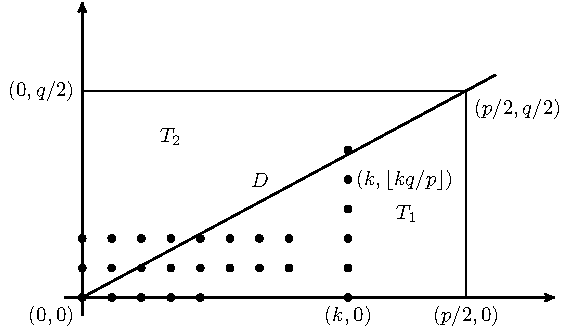
\includegraphics[scale=1]{figures/prf_qr.pdf} 	
  \caption{二次互反律的证明.}
  \label{fig:prf_qr}       % Give a unique label
  \end{center}
  \end{figure}
  
  现在可以开始二次互反律的证明。
  \begin{proof}[二次互反律的证明]
  首先，根据给定的素数$p$和$q$，构造如图~\ref{fig:prf_qr}所示的四边形，其四个顶点在坐标系中分别是$(0, 0)$，$(p/2, 0)$，$(0, q/2)$和$(p/2, q/2)$。
  证明的主体思路是分别使用两种不同的方法计算四边形中格点的个数，格点即坐标值为整数的点。
  因为$p$和$q$都是奇素数，所以四边形中的全部格点就是满足$1\leq m \leq (p-1)/2$，$1 \leq n \leq (q-1)/2$的$(m,n)$，其总数为：
  \[\frac{(p-1)}{2}\cdot \frac{(q-1)}{2}\]
  
  考虑四边形从坐标$(0,0)$到$(p/2, q/2)$的对角线$D$，其方程表达为$y = (q/p)x$，或者等价地表示为$py = qx$。因为$\gcd(p,q)=1$，所以四边形中所有
  格点都不会落在$D$上。记对角线$D$的上半部分为$T_2$，下半部分为$T_1$。先计算$T_1$中的格点数。对任意给定的$x$轴坐标值$1\leq k \leq (p-1/2)$，
  在$0 < y < kq/p$这个区间中的整数个数是$\left \lfloor kq/p \right\rfloor$。即在点$(k,0)$到$(k, kq/p)$这条垂线上的格点数为$\left \lfloor kq/p \right\rfloor$。
  所以下三角$T_1$中的格点个数为：
  \[ \sum_{k = 1}^{(p - 1)/2} \left \lfloor kq/p \right\rfloor\]
  同理，可计算上三角$T_2$中格点的个数为：
  \[ \sum_{j = 1}^{(q - 1)/2} \left \lfloor jp/q \right\rfloor\]
  因此，
  \[\frac{(p-1)}{2}\cdot \frac{(q-1)}{2}= \sum_{k = 1}^{(p - 1)/2} \left \lfloor kq/p \right\rfloor + \sum_{j = 1}^{(q - 1)/2} \left \lfloor jp/q \right\rfloor\]
  
  最后，利用推论~\ref{cor:gauss}，
  \begin{align*}
  \left(\frac{p}{q}\right) \left(\frac{q}{p} \right) 
  &= (-1)^{\sum_{j = 1}^{(q - 1)/2} \left \lfloor jp/q \right\rfloor} \cdot (-1)^{\sum_{k = 1}^{(p - 1)/2} \left \lfloor kq/p \right\rfloor }\\  
  &= (-1)^{\sum_{k = 1}^{(p - 1)/2} \left \lfloor kq/p \right\rfloor + \sum_{j = 1}^{(q - 1)/2} \left \lfloor jp/q \right\rfloor}\\
  &= (-1)^{((p-1)/2)((q-1)/2)}
  \end{align*}
 \qed
  \end{proof}
 %20200627
 \section{计算平方根}
 \label{sec:sqrt}
 在这一节，我们考虑这样一个问题。给定任意整数$n$，如何求解以下同余方程：
 \[x^ 2 \equiv a \pmod{n} \text{。}\]
 
 从简单情形开始考虑。如果同余式的模数是一个素数，则我们需要解的是：
 \[ x^2 \equiv a \pmod{p}\]
 
 
首先，需要判定该方程是否有解。运用欧拉准则，如果勒让德符号$\left( \frac{a}{p} \right) = 1$，方程有解，进入下一步骤。
否则，返回“无解”提示，程序结束。

接下来，我们要做的是“凑”一个平方数，它模$p$与$a$同余。思路是，给$a$乘上一个模$p$等于$1$的数，并且得到的值还能“凑”成一个平方数。
打断一下，这个提示能让读者回忆起中国剩余定理（定理~\ref{thm:crt}）的“重新发明过程”吗？
首先想到的应该是$a a^{-1}$，但是很快就会否决掉这个想法，因为这样乘上去什么都没有得到，还是一个$a$。那么找任意不等于$a$
的其他整数呢，比如，任取$b\in \Z$，乘$b b^{-1}$？也不行，因为不知道怎么凑出平方数。还是要乘一个与$a$相关（因为如果与$a$不相关，凑数将很困难），
且模$p$等于$1$的数，应该是什么？
建议大家在此掩卷思考几分钟，回忆最近的知识点中有没有这样的数值。

\begin{thinking}
根据费尔马小定理，$a^{p-1} \equiv 1 \pmod{p}$，似乎也满足我们的需求。给$a$乘上$a^{p-1}$能不能带来好的结果呢？
为什么或者为什么不？
\end{thinking}

在把$a^{p-1} \equiv 1 \pmod{p}$否定掉之后，现在应该想起，勒让德符号$\left( \frac{a}{p} \right) = 1$，根据欧拉准则，即有$a^{(p-1)/2} \equiv 1 \pmod{p}$。
于是很高兴地发现：
 \[a \equiv a^{(p-1)/2}\cdot a \equiv a^{(p+1)/2} \equiv (a^{(p+1)/4})^2  \pmod{p} \]
$a^{(p+1)/4} $似乎就是我们需要的答案。不过，且慢，请问$(p+1)/4$一定是整数？如果是，那么求解就成功了。
所以，倒不如问，在什么情况下$(p+1)/4$一定是整数？

要使得$(p+1)/4$为整数，就是需要存在$k \in \Z$，使得$(p + 1) = 4k$。简单的计算可知，
其实就是要求$p \equiv -1 \pmod{4}$，或者写成$p \equiv 3 \pmod{4}$。
所以，如果$p$满足模$4$余$3$，则同余方程有解$\pm a^{(p+1)/4}$。
使用代码表示以上分析如下：
\begin{lstlisting}[language=Python]
Input: 整数a和p
Output: 求x使得x^2 模p与a同余
def find_sqrt(a, p):
    assert (p + 1) % 4 == 0   # p mod 4 余 3;
    assert is_prime(p)         # p 为素数;
    if legendre_symbol(a, p) != 1: return []   #勒让德符号不为1则无解;
    b = (p + 1) // 4
    return [a^b % p, -a^b % p ] 
\end{lstlisting}
 
 如果$n = pq$，且$p$和$q$都是满足$p \equiv q \equiv 3 \pmod{4}$的素数，
 解同余方程$ x^2 \equiv a \pmod{n}$等价于先解以下两个模素数的同余方程。
\begin{align*}
 x^ 2 &\equiv a \pmod{q} \\
 x^2 &\equiv a \pmod{p}
 \end{align*}
 然后，使用中国剩余定理可以找到所有解。至于模$4$余$1$的情形，则暂且不讨论。
 
 %%2023年6月12日
 \section*{章注}
 %\section*{Chapter Note}
 \addcontentsline{toc}{section}{章注}
 读者往往很轻易地就会惊叹于二次剩余相关知识的理论高度，特别是在得知高斯对二次互反律的天才论断，以及知道二次互反律已有超过200种不同的的证明\footnote{出自\href{https://zh.wikipedia.org/zh-sg/二次互反律}{维基百科}。}之后。
 
 可能读者目前还不知道的是，二次剩余也有着丰富的应用，无论是在理论上或实践中。在20世纪80年代，美国麻省理工学院教授 Shafi Goldwasser 和 Silvio Micali
 提出了一种概率加密算法~\cite{GM84}，该算法以二次剩余为理论基础。
 另外，Goldwasser 等人还天才地利用二次剩余的理论提出了一种交互式零知识证明系统~\cite{GMR89}。这些工作对计算机科学理论、现代密码学等领域
 产生了深远的影响，值得读者关注。因此，Goldwasser 和 Micali 获得了2012年的图灵奖。
 
 \begin{problemset}
 \item 请计算以下勒让德符号：$(\frac{7}{11})$，$(\frac{72}{131})$，$(\frac{20}{23})$，$(\frac{17}{31})$。%-1， -1， -1，-1
 
 \item 使用群论的第一同构定理证明定理~\ref{thm:num_qr}。
 
 \item 证明命题~\ref{pro:QR_gr}。
 
 \item 定义映射$\psi\colon \Z_p^* \to \{ \pm 1 \}$
  为$\psi(a) =  \left(\frac{a}{p}\right)$，$\forall a \in \Z_p^*$。请证明这是一种满同态。[提示：$\{ \pm 1 \}$在乘法上成群。]
 
 \item 证明命题~\ref{pro:leg_sym}。
 
 \item 给出推论~\ref{cor:qu_rec}的完整证明。
 
 \item 设$p$是奇素数，请证明$\Z_p^*$的所有生成元都是模$p$的二次非剩余。%应用欧拉准则立得！
  
 \item 使用抽象代数的语言重新证明欧拉准则。
 
 \item  利用二次互反律，写程序完成$\left(\frac{q}{p}\right)$的计算，$p$和$q$是任意的奇素数。
 
 \item 设$n = 7 \cdot 11$，请手动计算求出同余方程$x^2 \equiv a \pmod{n}$在$a = 5$和$a = 4$时的所有解。%ans，a = 5时无解: 
 
 \item 构思算法并写成一个程序求解同余方程$x^2 \equiv -1 \pmod{p}$，其中，$p$是模$4$余$1$的素数。
 % 源自Jar14，使用欧拉准则，求a使得a^(p-1)/2 = -1，那么x=a^(p-1)/4. 20250911
 
 \item 写一个程序求解同余方程$x^2 \equiv a \pmod{n}$，其中要求$n = pq$，且$p$和$q$是模$4$余$3$的两个不同素数。 
 
 \item 对大于$2$的素数$ p $计算$2^{(p-1)/2} \bmod p$，根据计算结果找规律，并形成自己的猜想，最后给出证明。
 
 \item 二次探测（quadratic probing）法是 hash 表解决冲突的一种常用策略。一种命名为 alternating signs 的 hash 函数的定义方式如下。
 设哈希表长度为一个模$4$余$3$的奇素数 $p$，初始哈希地址为$\operatorname{H}(k) \in \Z_p$。定义第$i$次探测位置为：
 \[\operatorname{H}(k,i) \equiv \operatorname{H}(k) + (-1)^{(i+1)} \cdot i^2 \pmod{p}\]，其中$i\in \Z_p$。使用$i=0$ 表示初始探测位置，因此$\operatorname{H}(k, 0) = \operatorname{H}(k)$。
 请分析证明为什么需要取一个模$4$余$3$的素数$p$。
 
 \end{problemset}
 
 
